
\documentclass[10pt,a4paper]{article}
\usepackage[margin=2.0cm]{geometry}
\usepackage{amsmath,amssymb,booktabs,longtable,graphicx,float,hyperref,xcolor,array}
\hypersetup{colorlinks=true,linkcolor=blue,urlcolor=blue,citecolor=blue}
\title{Auditable Hierarchical Alpha Ensembling for A-Share Cross-Sectional Prediction\\
\large Strict IS/OOS Separation, Correlation-Constrained Greedy Selection, and Matrix-Level Nesting}
\author{YYB Quantitative Research Platform}
\date{Generated from frozen evidence: 2026-06-02T00:46:52}
\begin{document}
\maketitle

\begin{abstract}
We study cross-sectional prediction of five-day A-share returns using a local research platform with strict
in-sample (IS, 2020--2022) selection and out-of-sample (OOS, 2023) evaluation. The frozen audit compares
equal weighting, ICIR weighting, and inverse-volatility shrinkage across unfiltered and correlation-constrained
baskets; five neutralization regimes; and exploratory matrix-level hierarchical nesting. The best confirmatory
configuration is \texttt{top\_is\_sharpe\_n5\_icir\_beta} with OOS Sharpe 12.882.
We additionally apply a hard portfolio screen requiring Sharpe $>10$ and pairwise absolute daily-PnL
correlation $<0.5$. The requested portfolio of ten candidates is not satisfied: only 1 candidates pass both constraints. We report this shortfall directly rather than fill the target with
economically redundant variants. All headline tables and figures are generated from a single frozen JSON
artifact, and exploratory nested results are separated from confirmatory evidence.
\end{abstract}

\section{Research question and contributions}
The empirical question is whether economically interpretable A-share signals can be combined into robust,
low-redundancy predictors under strict temporal separation. The platform contributes: (i) an auditable IS/OOS
protocol; (ii) true PnL-correlation greedy selection rather than family-name proxies; (iii) five explicit
neutralization regimes; and (iv) matrix-level nesting in which a cached OOS combo matrix can become an input to
a higher-level combo without reparsing its leaves. The audit also records negative results, skipped features,
and missing infrastructure rather than silently excluding them.

\section{Data and validation protocol}
The local panel contains 970 trading days, 5,515 A-share securities, and 89 raw or derived fields. The target is
the future five-day return. IS spans 2020--2022 and is used for ranking and weight estimation; OOS spans 2023
and is used only for evaluation. Correlation screening converts cumulative PnL to daily changes and uses
absolute Pearson correlation. The confirmatory matrix is frozen before ranking OOS results. Exploratory L1--L3
nesting is explicitly labelled exploratory because its layer choices inspect OOS outcomes.

\paragraph{Trading-protocol limitation.}
The current research engine excludes immature listings and ST securities, but it does not yet model all
execution frictions needed for a production claim: commissions, stamp duty, market impact, limit-up/down
execution, T+1 constraints, and capacity. Reported Sharpe ratios are therefore signal-research metrics, not
deployable net-performance claims.

\section{Combination methods}
For standardized cross-sectional signals $z(F_i)$, the linear combo is
\[
F_c = \sum_{i=1}^N w_i z(F_i).
\]
Equal weighting uses $w_i=1/N$. ICIR weighting uses IS rank-IC stability,
$w_i \propto \max(0.1,\mathrm{ICIR}_i^{IS})$. The platform's historical ``ridge'' label is retained in
tables for compatibility, but the implementation is accurately described as inverse-volatility shrinkage:
$w_i \propto 1/(\sigma_i^{IS}+\mathrm{median}(\sigma^{IS}))$. It is not a standard ridge-regression
optimizer. LightGBM is an exploratory nonlinear benchmark and is not mixed into the confirmatory table.

\section{Neutralization ablation}
The audit evaluates: no neutralization; market-cap decile demeaning; cross-sectional log-market-cap regression;
cross-sectional beta regression; and joint log-market-cap plus beta regression. Reliable industry labels are
not available in the current data catalog, so industry neutralization is not fabricated. Figure~\ref{fig:neutral}
reports mean Sharpe changes relative to the unneutralized control.

\begin{figure}[H]\centering
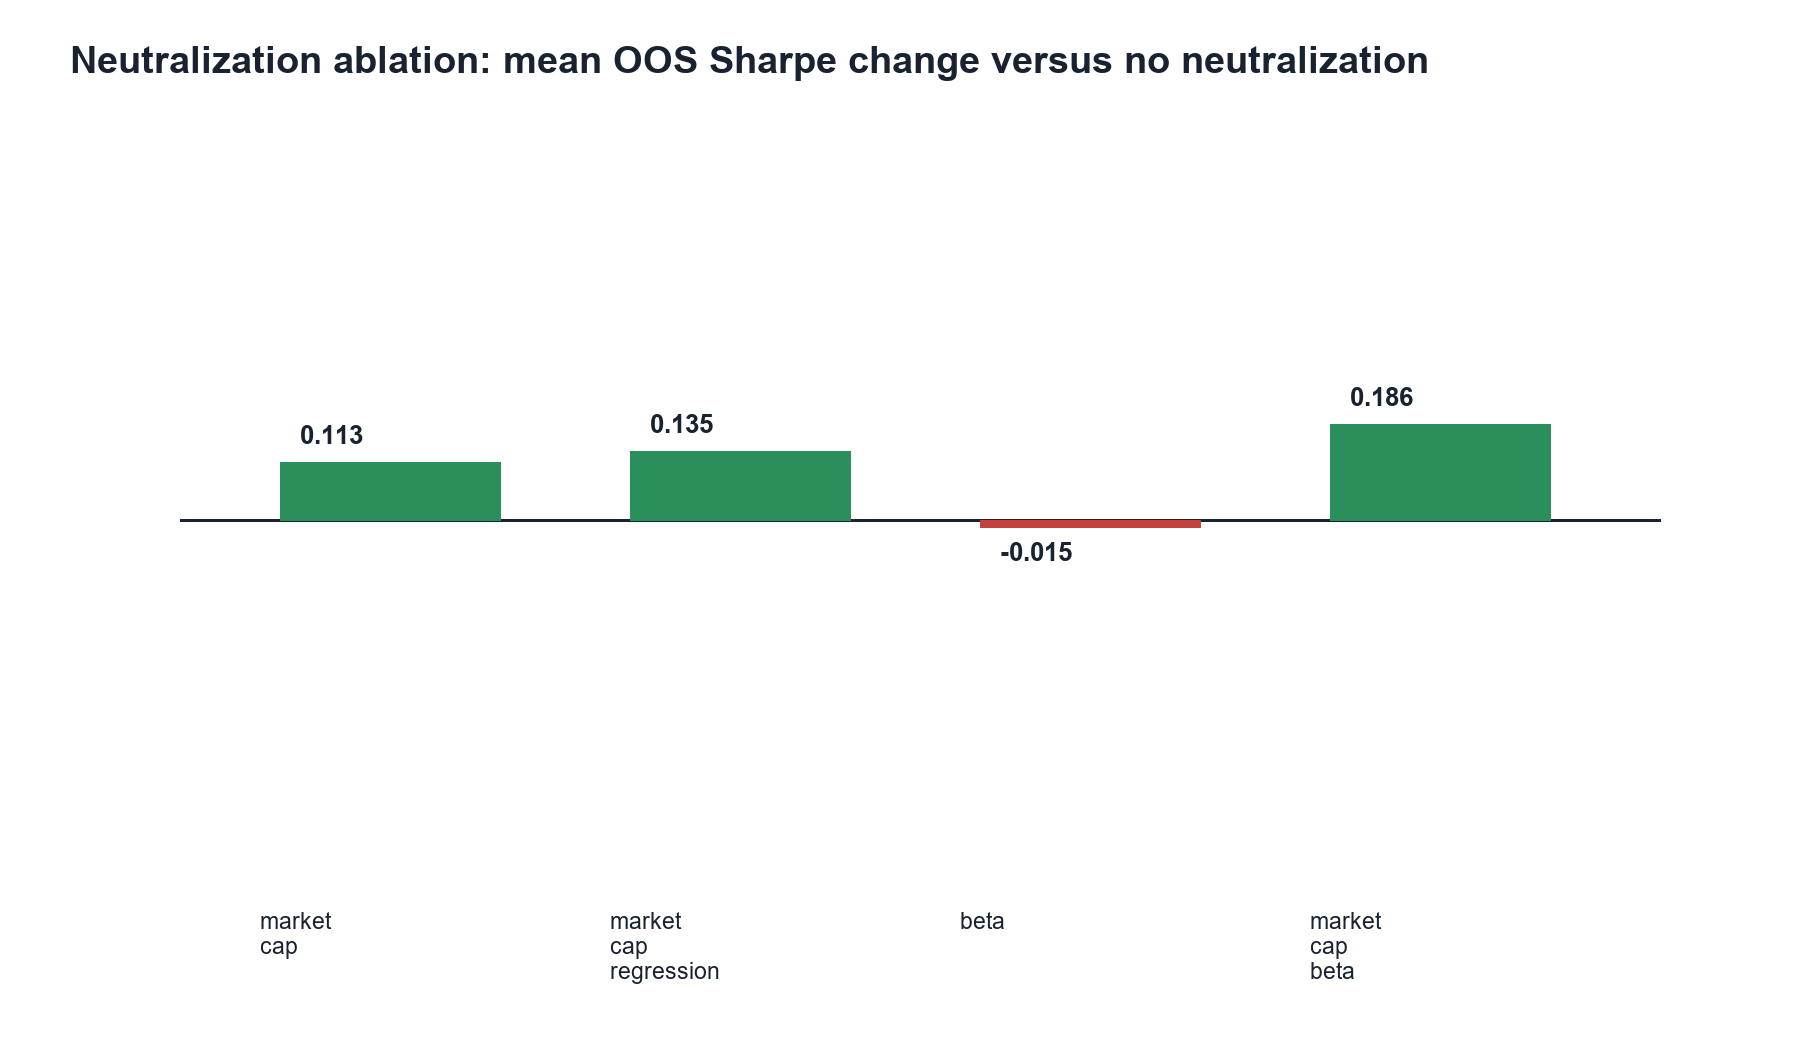
\includegraphics[width=0.95\linewidth]{figures_final/neutralization_ablation.png}
\caption{Neutralization ablation using frozen confirmatory baskets.}\label{fig:neutral}
\end{figure}

\section{Confirmatory results}
\begin{figure}[H]\centering
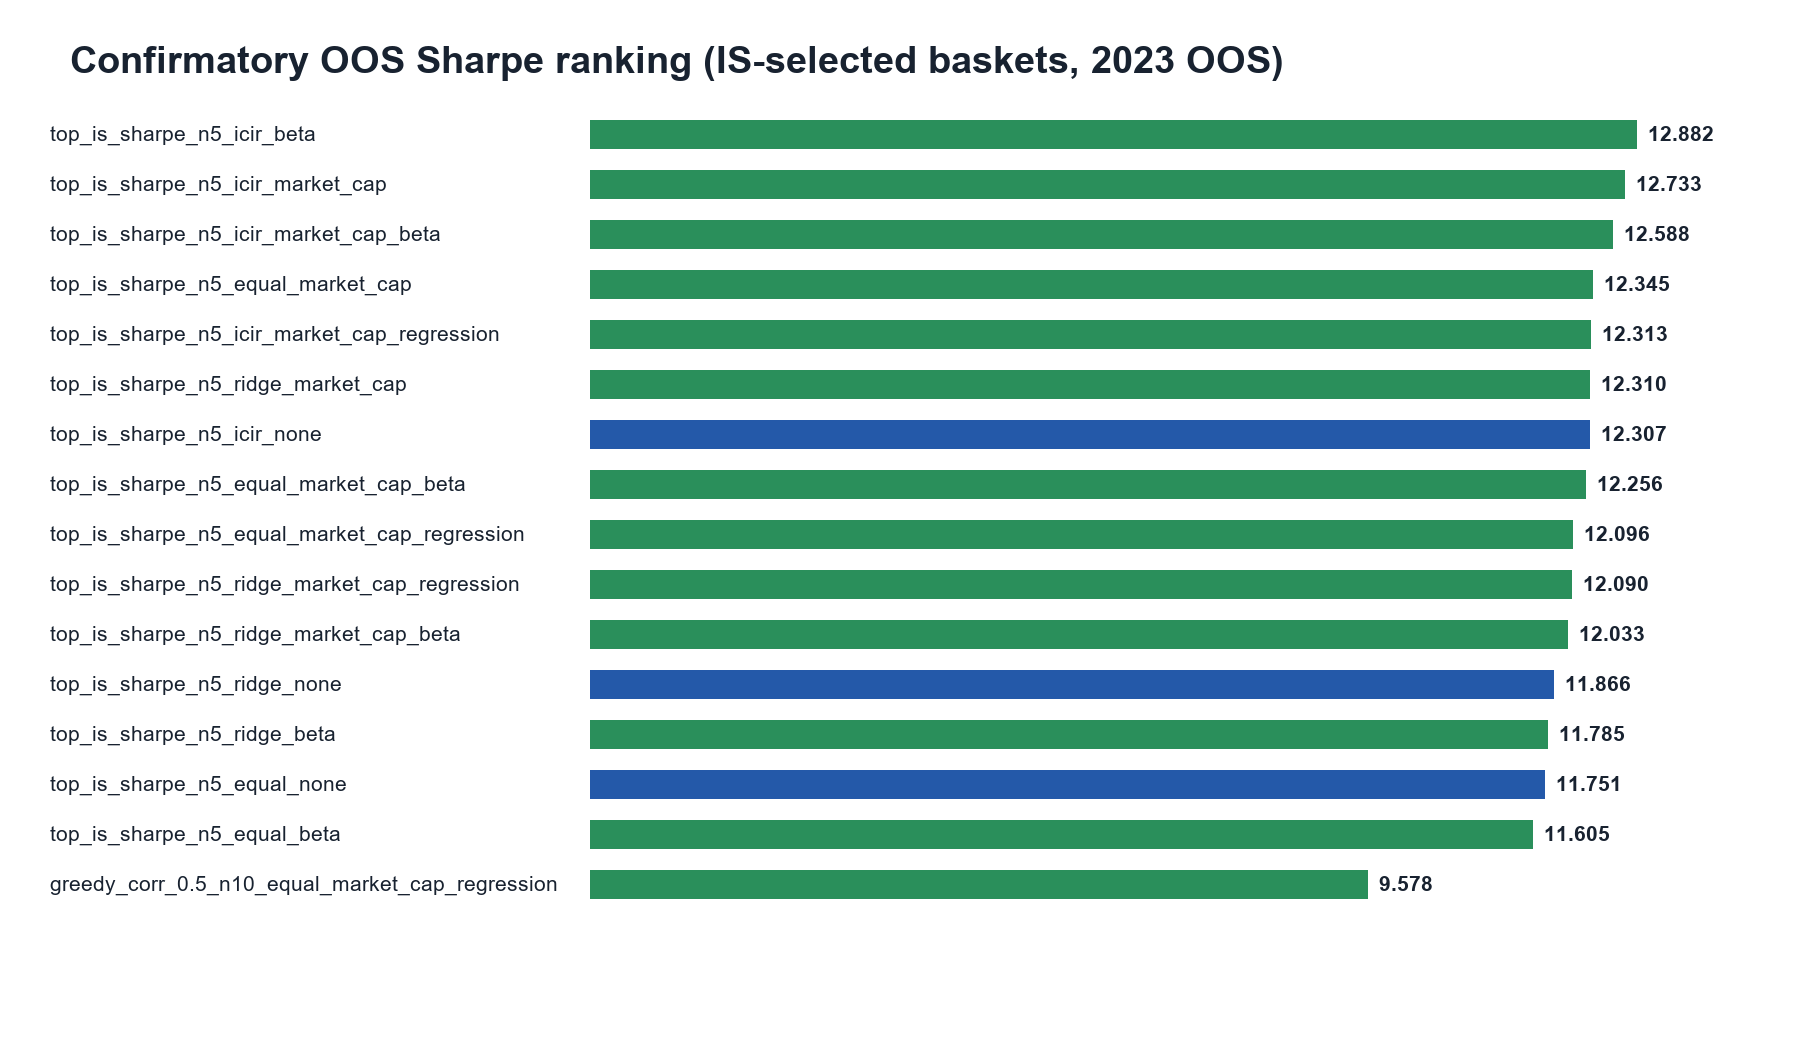
\includegraphics[width=0.98\linewidth]{figures_final/confirmatory_sharpe.png}
\caption{Top confirmatory OOS Sharpe values. Baskets and weights are selected using IS information only.}
\end{figure}

\begin{table}[H]\centering\small
\caption{Top frozen confirmatory configurations.}
\begin{tabular}{r l r r r}
\toprule Rank & Configuration & Sharpe & IC & Turnover \\
\midrule
1 & top\_is\_sharpe\_n5\_icir\_beta & 12.882 & 0.0402 & 0.2709 \\
2 & top\_is\_sharpe\_n5\_icir\_market\_cap & 12.733 & 0.0396 & 0.2695 \\
3 & top\_is\_sharpe\_n5\_icir\_market\_cap\_beta & 12.588 & 0.0402 & 0.2701 \\
4 & top\_is\_sharpe\_n5\_equal\_market\_cap & 12.345 & 0.0401 & 0.2400 \\
5 & top\_is\_sharpe\_n5\_icir\_market\_cap\_regression & 12.313 & 0.0395 & 0.2696 \\
6 & top\_is\_sharpe\_n5\_ridge\_market\_cap & 12.310 & 0.0406 & 0.2834 \\
7 & top\_is\_sharpe\_n5\_icir\_none & 12.307 & 0.0395 & 0.2698 \\
8 & top\_is\_sharpe\_n5\_equal\_market\_cap\_beta & 12.256 & 0.0411 & 0.2465 \\
9 & top\_is\_sharpe\_n5\_equal\_market\_cap\_regression & 12.096 & 0.0400 & 0.2444 \\
10 & top\_is\_sharpe\_n5\_ridge\_market\_cap\_regression & 12.090 & 0.0403 & 0.2856 \\
11 & top\_is\_sharpe\_n5\_ridge\_market\_cap\_beta & 12.033 & 0.0409 & 0.2858 \\
12 & top\_is\_sharpe\_n5\_ridge\_none & 11.866 & 0.0406 & 0.2800 \\
\bottomrule
\end{tabular}
\end{table}

\begin{figure}[H]\centering
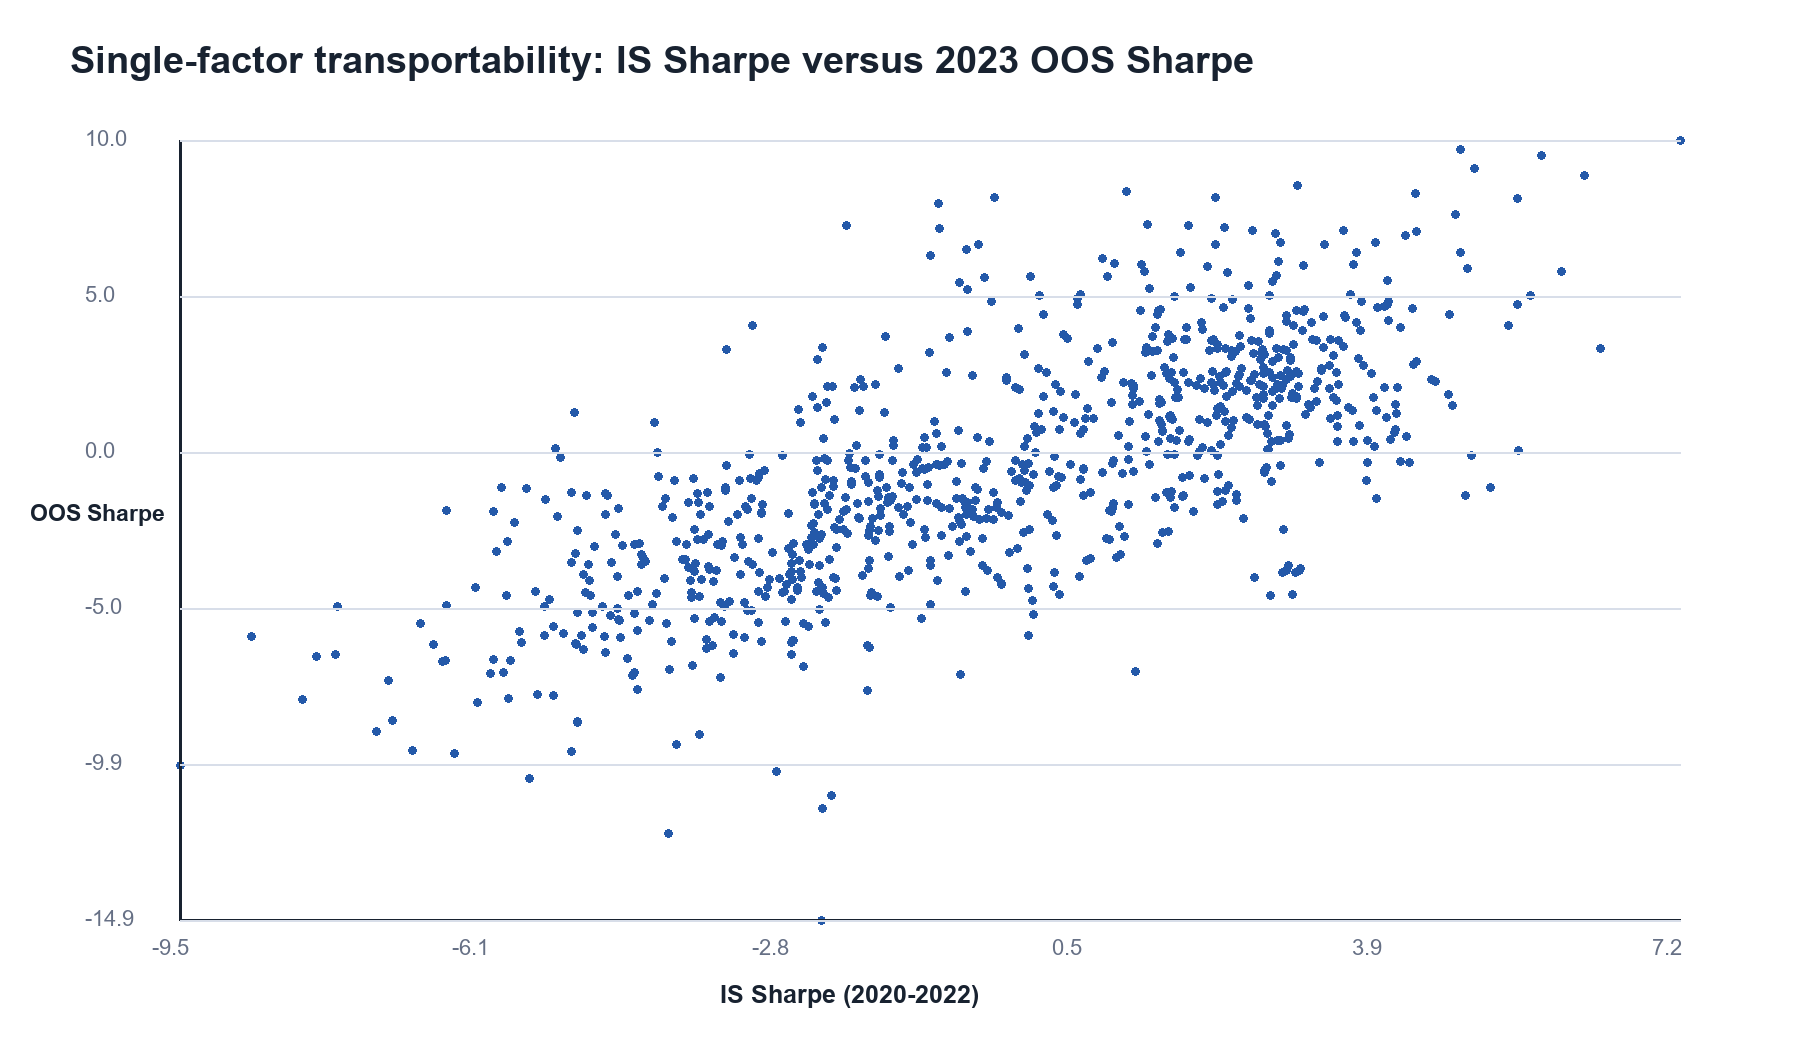
\includegraphics[width=0.92\linewidth]{figures_final/is_oos_scatter.png}
\caption{Single-factor IS Sharpe versus 2023 OOS Sharpe. Dispersion motivates explicit OOS isolation and
economic screening.}
\end{figure}

\section{Correlation-constrained target portfolio}
The delivery target is ten factors with Sharpe $>10$ and pairwise absolute daily-PnL correlation $<0.5$.
The screen is hard: no relaxation and no duplicate PnL curves are admitted. The requested portfolio of ten candidates is not satisfied: only 1 candidates pass both constraints.

\begin{table}[H]\centering\small
\caption{Strict high-Sharpe, low-correlation screen.}
\begin{tabular}{r l r r r r r}
\toprule Rank & ID prefix & Sharpe & IC & Fitness & Turnover & Max corr. \\
\midrule
1 & d88b1b68-724 & 13.351 & 0.0433 & 18.316 & 0.3161 & 0.0000 \\
\bottomrule
\end{tabular}
\end{table}

\begin{figure}[H]\centering
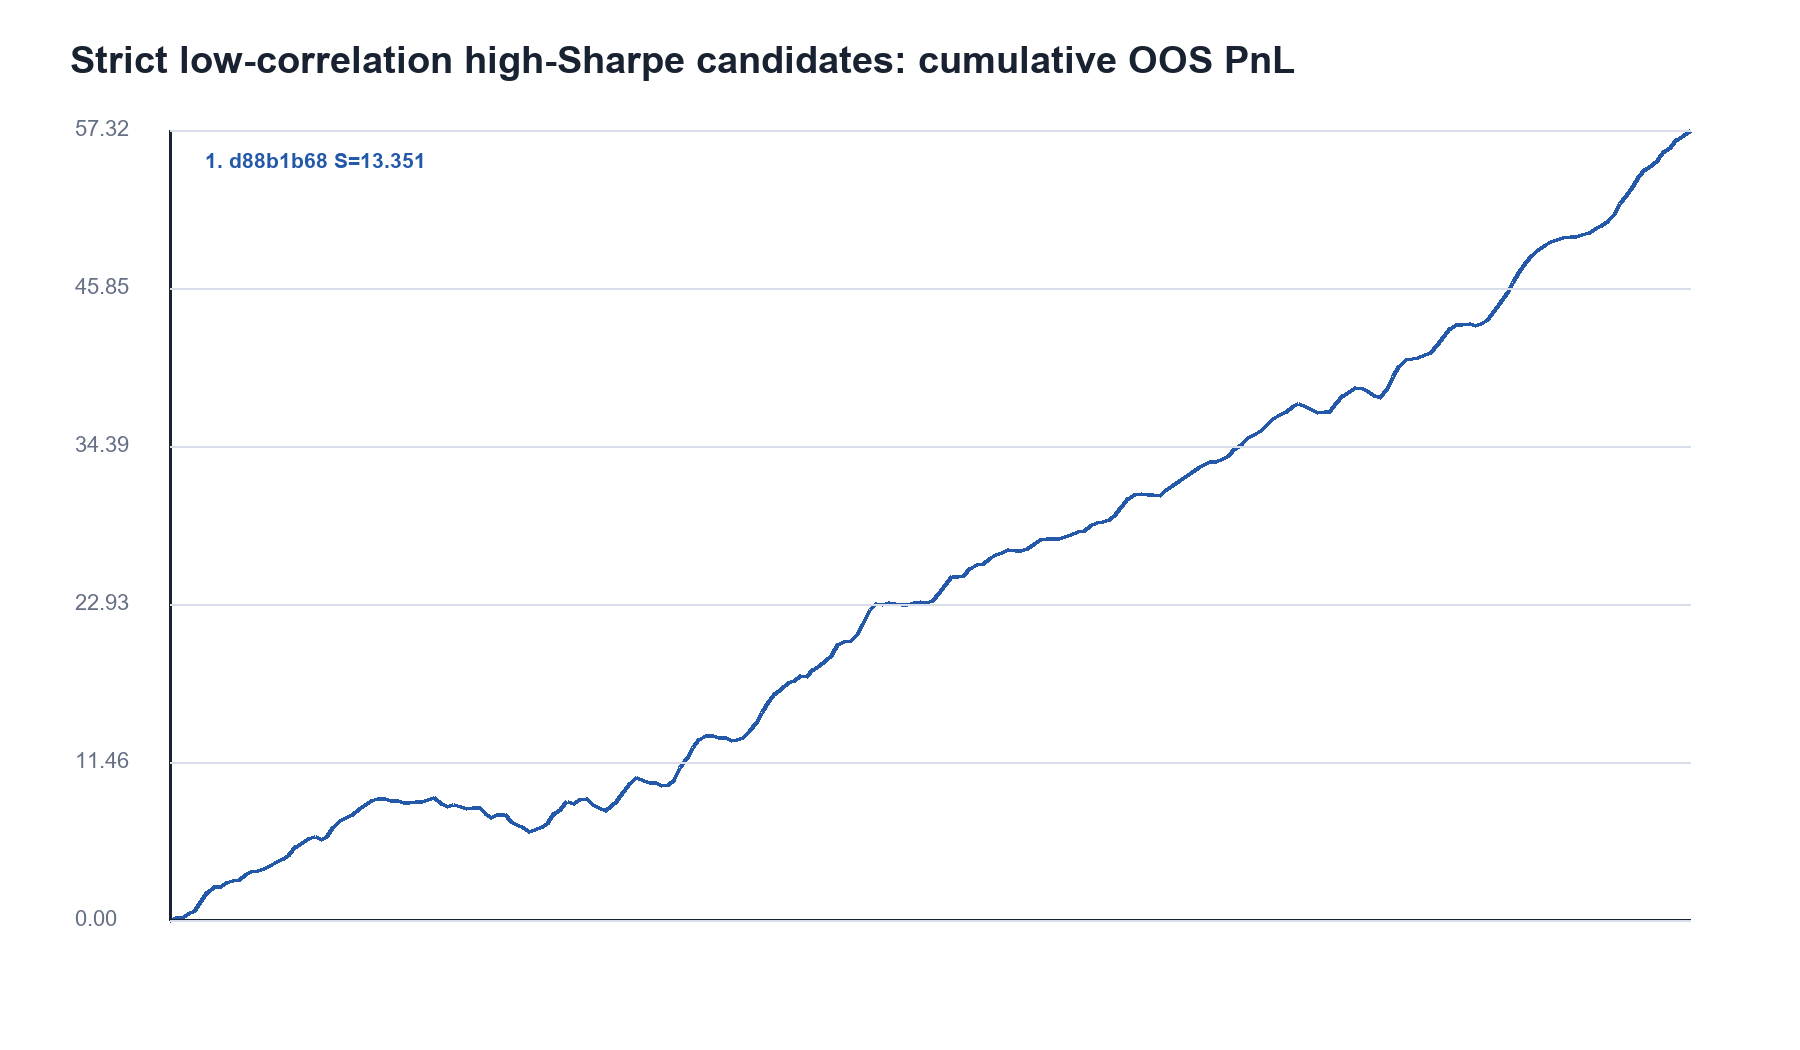
\includegraphics[width=0.95\linewidth]{figures_final/strict_candidate_curves.png}
\caption{Cumulative OOS PnL curves for strict candidates.}
\end{figure}
\begin{figure}[H]\centering
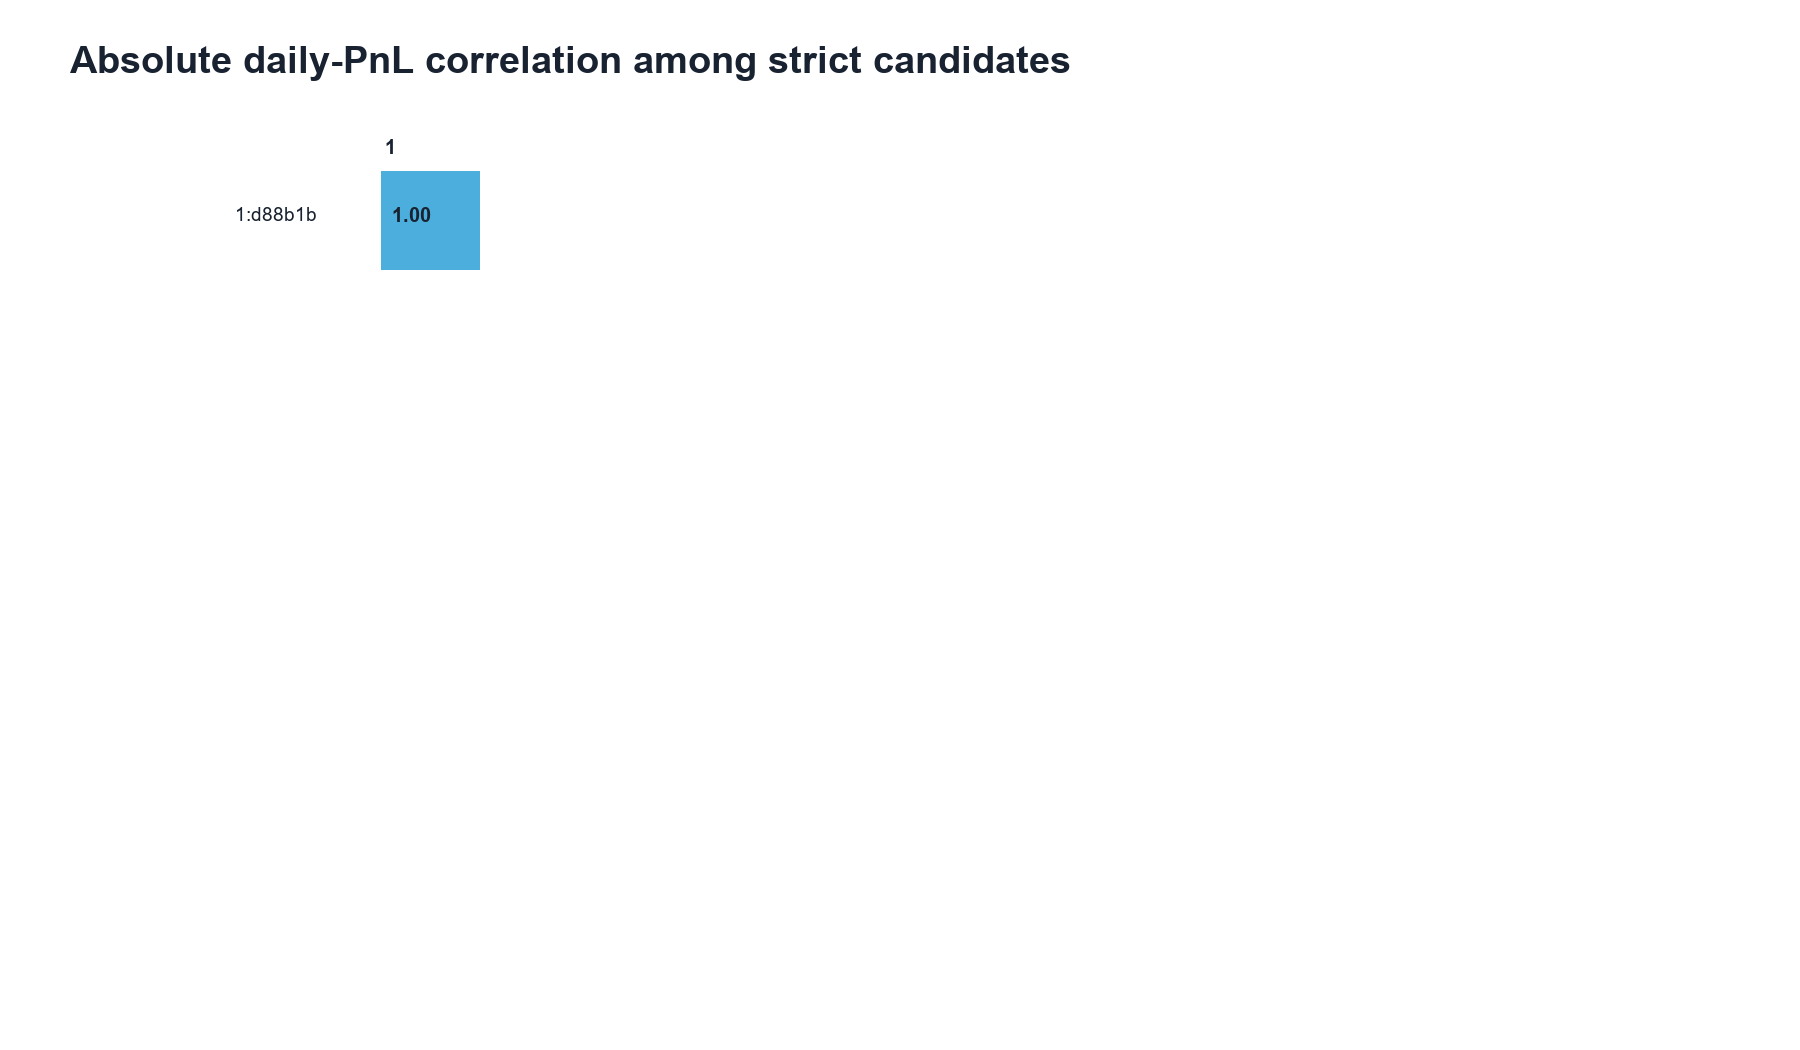
\includegraphics[width=0.78\linewidth]{figures_final/strict_correlation_heatmap.png}
\caption{Absolute daily-PnL correlation heatmap for strict candidates.}
\end{figure}

\subsection{Economic interpretation of strict candidates}
Each surviving strict candidate is an ensemble rather than an atomic anomaly. The table reports its dominant
economic interpretation and detected child proxies. For new nested records, child lookup follows preserved
\texttt{superalpha\_ref(...)} lineage recursively. For legacy cached records, the stored expression is inspected
directly and missing leaf labels are reported rather than invented.

\begin{longtable}{r l p{5.0cm} p{6.0cm}}
\toprule Rank & ID prefix & Ensemble interpretation & Detected child proxies \\
\midrule
1 & d88b1b68-724 & composite cross-sectional signal & legacy composite; leaf labels unavailable \\
\bottomrule
\end{longtable}

\section{Economic interpretation of the frozen greedy seed basket}
The correlation-constrained seed basket is not presented as a causal structural model. It is an interpretable
set of cross-sectional proxies used to construct candidate ensembles. Liquidity terms proxy crowding and
trading frictions; return terms proxy continuation or overreaction; reversal and auction terms proxy short-lived
price pressure; risk terms condition exposure on the volatility regime; and intraday terms describe price
formation. Each leaf remains inspectable in the frozen manifest.

\footnotesize
\begin{longtable}{r >{\raggedright\arraybackslash}p{4.7cm} >{\raggedright\arraybackslash}p{5.4cm} r r}
\toprule Rank & Leaf expression & Economic interpretation & IS Sharpe & OOS Sharpe \\
\midrule
1 & \path{-rank(log_dollar_vol) - rank(ret_120d_s...} & liquidity and crowdedness; medium-horizon continuation or reversal & 7.209 & 9.960 \\
2 & \path{-rank(abs(zscore(turnover_5d) - zscore(...} & liquidity and crowdedness & 6.327 & 3.331 \\
3 & \path{zscore(ret_20d) - zscore(turnover_rate)} & liquidity and crowdedness; medium-horizon continuation or reversal & 6.153 & 8.869 \\
4 & \path{-rank(log_dollar_vol) - rank(ret_20d)} & liquidity and crowdedness; medium-horizon continuation or reversal & 5.894 & 5.787 \\
5 & \path{-rank(abs(zscore(turnover_rate)))} & liquidity and crowdedness & 5.668 & 9.484 \\
6 & \path{-rank(abs(zscore(turnover_rate) - zscor...} & liquidity and crowdedness & 5.547 & 5.024 \\
7 & \path{-rank(abs(zscore(turnover_rate) - zscor...} & liquidity and crowdedness; risk-regime conditioning & 5.410 & 0.085 \\
8 & \path{-rank(abs(zscore(turnover_5d) - zscore(...} & liquidity and crowdedness; risk-regime conditioning & 5.403 & 8.120 \\
9 & \path{-rank(abs(ret_20d - abnormal_vol_rev))} & medium-horizon continuation or reversal; risk-regime conditioning & 5.103 & -1.073 \\
10 & \path{-rank(abs(zscore(turnover_5d) - zscore(...} & liquidity and crowdedness; short-horizon overreaction correction & 4.852 & 5.900 \\
\bottomrule
\end{longtable}
\normalsize

\subsection{Child-factor economic dictionary}
The following dictionary explains the detected leaf proxies used by the strict candidates and frozen greedy
seed basket. Operators such as ranking, z-scoring, absolute deviation, and signed aggregation change scaling or
interaction shape; they do not create a new economic primitive.

\begin{longtable}{p{3.6cm} p{11.2cm}}
\toprule Child proxy & Economic interpretation \\
\midrule
abnormal\_vol\_rev & abnormal-volume reversal; a short-lived price-pressure proxy \\
amihud\_20d & Amihud illiquidity; price impact per traded value \\
log\_dollar\_vol & log trading-value scale; a liquidity, capacity, and crowding proxy \\
ret\_120d\_skip5 & longer-horizon return excluding the most recent week; persistent trend proxy \\
ret\_20d & medium-horizon return; continuation versus reversal state \\
turnover\_5d & short-horizon turnover intensity; a transient liquidity-demand proxy \\
turnover\_rate & share turnover intensity; a trading-pressure and crowdedness proxy \\
volume\_profile\_ratio & relative volume-shape abnormality; an intraday participation proxy \\
\bottomrule
\end{longtable}

\section{Exploratory hierarchical nesting}
Matrix-level nesting caches each OOS combo matrix and reuses it as a higher-level input. New records preserve
lineage through \texttt{superalpha\_ref(history-id)} references while loading the corresponding cached matrix.
This is an engineering contribution and an exploratory modeling result: selecting the best lower layer after
viewing OOS performance is not confirmatory evidence.

\begin{figure}[H]\centering
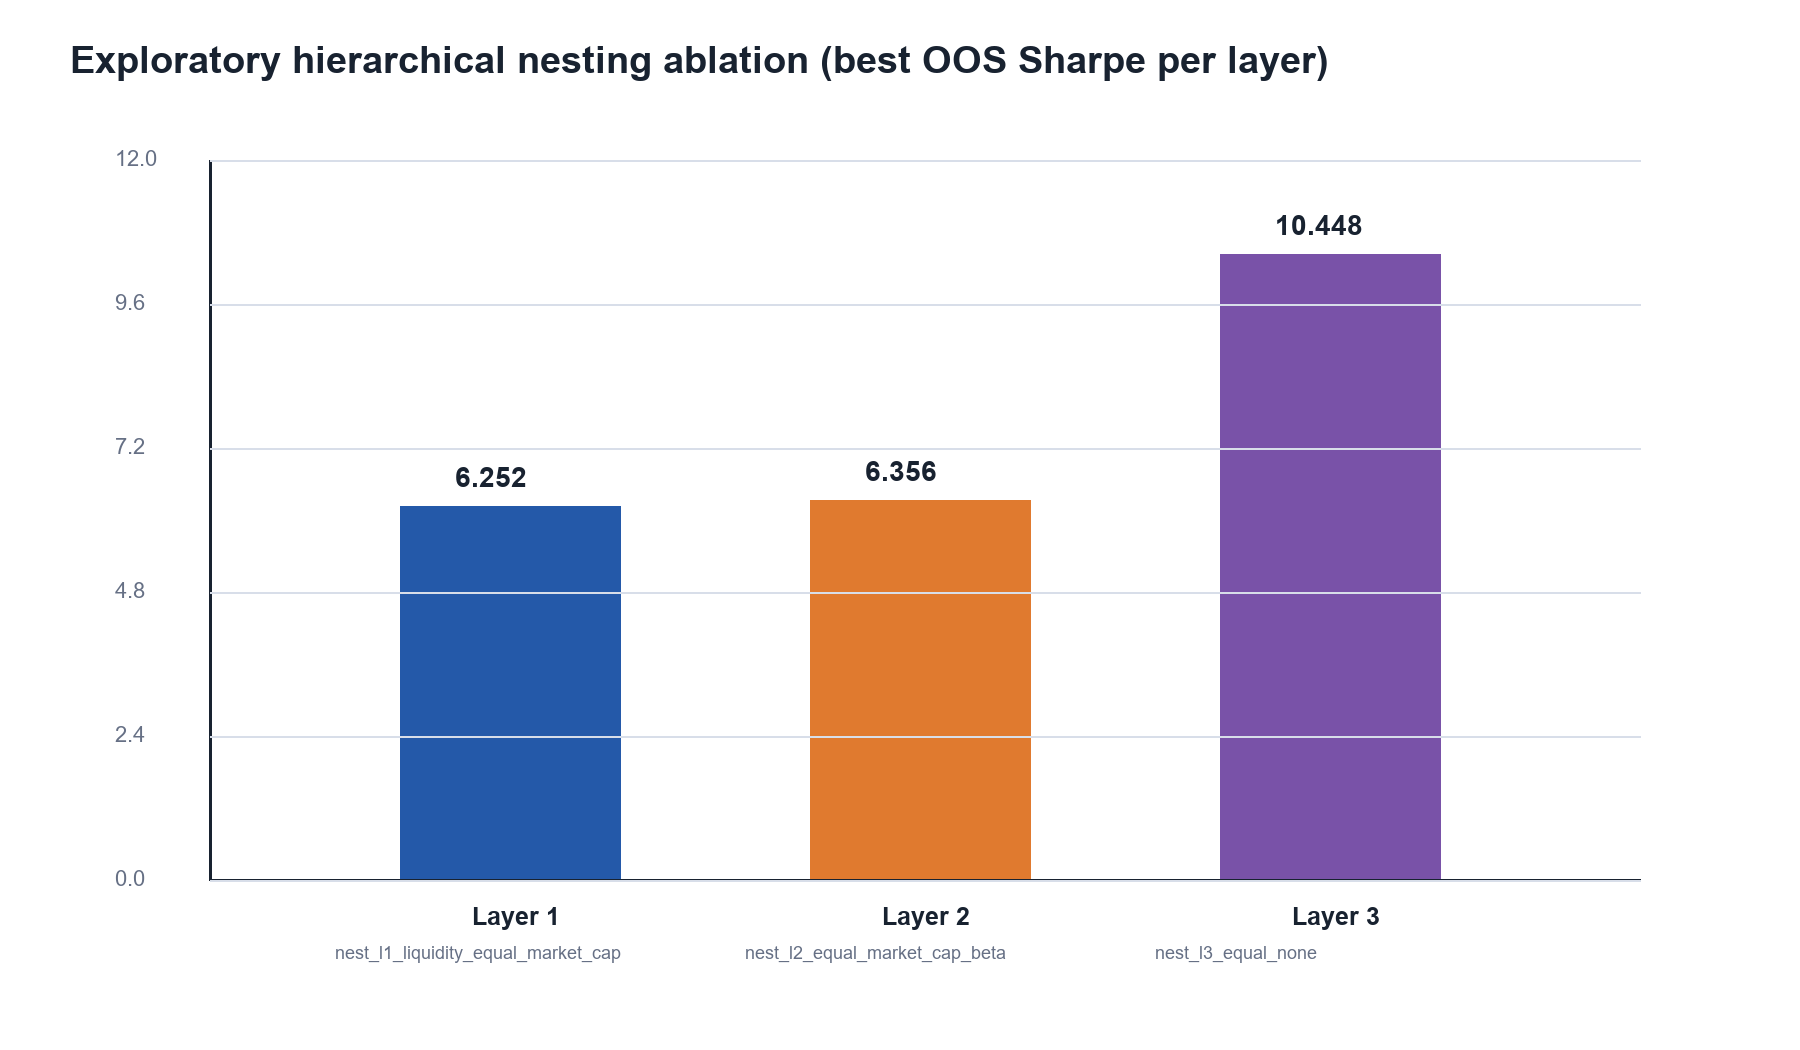
\includegraphics[width=0.88\linewidth]{figures_final/nesting_ablation.png}
\caption{Exploratory L1--L3 nesting ablation.}
\end{figure}

\section{Threats to validity}
\begin{enumerate}
\item The OOS window contains one calendar year. A publishable asset-pricing claim requires multi-period
walk-forward validation and regime splits.
\item Transaction costs, delay sensitivity, T+1 execution, price limits, and capacity remain to be integrated.
\item The factor search space is large. Multiple testing is controlled operationally by IS-only selection and
frozen OOS reporting, but formal false-discovery analysis remains future work.
\item Historical cached combos created before lineage preservation remain valid matrices but cannot support
leaf-level economic attribution. They are marked as legacy artifacts.
\item Industry neutralization is absent because reliable industry labels are unavailable in the current snapshot.
\end{enumerate}

\section{Reproducibility}
The frozen evidence file is \path{experiment_results/final_audit_results.json}. The runner is
\path{run_final_audit_experiments.py}. Every confirmatory row stores input IDs, weighting method,
neutralization mode, requested and valid feature counts, skipped features, metrics, and PnL. The Flask service
remains available for remote read-only review throughout the audit; external Alpha submission is outside the
scope of this work.

\section{Conclusion}
The final audit replaces an earlier narrative report with a reproducible evidence chain. The main empirical
lesson is not that arbitrary stacking guarantees high Sharpe. Rather, strict temporal separation, explicit
neutralization, and true PnL-correlation constraints expose how quickly superficially strong variants collapse
into the same economic bet. Matrix-level nesting remains useful, but only when its lineage and exploratory
status are preserved.

\begin{thebibliography}{9}
\bibitem{debondt1985} De Bondt, W. and Thaler, R. (1985). Does the stock market overreact? \emph{Journal of Finance}.
\bibitem{jegadeesh1993} Jegadeesh, N. and Titman, S. (1993). Returns to buying winners and selling losers. \emph{Journal of Finance}.
\bibitem{fama1993} Fama, E. and French, K. (1993). Common risk factors in the returns on stocks and bonds. \emph{Journal of Financial Economics}.
\bibitem{harvey2016} Harvey, C., Liu, Y., and Zhu, H. (2016). ... and the cross-section of expected returns. \emph{Review of Financial Studies}.
\bibitem{gu2020} Gu, S., Kelly, B., and Xiu, D. (2020). Empirical asset pricing via machine learning. \emph{Review of Financial Studies}.
\end{thebibliography}
\end{document}
